In order to structure the UX evaluation we created the following testplan, which is also meant to focus the evaluation and define milestones in the further development of the product.

\subsection{Testplan}
Our evaluation is formative, as our goal is to improve Amazon. \\ \\
\textbf{Purpose:} We want to test the user's experience and satisfaction of Amazon, both pragmatically and hedonically.

\newpage
\textbf{Main questions:}
\begin{itemize}
\item Are there parts of the system the user is not satisfied with?
\item Which parts of the system did the user not use?
\item Are there parts of the system that is troublesome to the user?
\end{itemize}
\textbf{User profile:}
Ordinary Danes without a technical background. \\ \\
\textbf{Users and roles:}
One of us will function as a moderator and the other will be taking notes. Also our users are required to be capable of cooperating. \\ \\
\textbf{Test methods:}
\begin{itemize}
\item Questionares : AttrakDiff
\item Lab studies : Co-discovery
\end{itemize}
\textbf{Assignments:} The assignments are generally structured as stories with the intention of making the user explore the system, without guiding the user and keeping interaction with the user minimal. Examples of the stories used can be seen in \autoref{appendix:codiscovery} \\ \\
\textbf{Context and equipment:} In the context of the lab study we make use of the internet, a laptop for the users to use, a projector to be able to observe their interaction with the system during the evaluation, assignments to be solved by the users and a questionare in paper format. \\ \\
\textbf{Data collection:} Data is collected through the questionare and notes taken during the lab study. \\

As is pointed out in Hassenzahl Funology (2003) \citep{Hassenzahl2003}, a consumer's experience, and perception, of a product is very much shaped by not only its pragmatic features, but largely also  by hedonic features. Hassenzahl also introduces a model for placing the product based on its pragmatic and hedonic features, see \autoref{hassenzahl} below.

\begin{figure}[h]
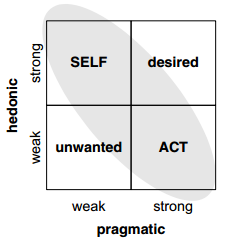
\includegraphics[scale=0.55]{includes/hassenzahl.png}
\caption{Pragmatic vs hedonic product scale}
\label{hassenzahl}
\end{figure}
Amazon is located in the ACT box, meaning that it is heavily pragmatically focused. 

\subsection{Description of evaluation process}
The evaluation of the system is done with a total of two participants, both male.

In order to evaluate the system we combine the two methods in the following manner: The two participants are present in the lab simultaneously, and are first read aloud an introduction detailing the purpose, and expectations, of the evaluation. The document specifying this can be found in \autoref{appendix:introductiontext}. They are then asked to sign a document specifying that they understand and accept the terms and conditions of the evaluation, see \autoref{appendix:codiscovery}.
The evaluation is now started using co-discovery, which the participants began by reading the current assignment aloud. While in the process of solving the assignments they were thinking aloud, and notified the moderator when they thought they had finished an assignment. The expected time of completion for co-discovery was 40 minutes, while the actual evaluation lasted only 17 minutes.

When the participants had solved all the assignments they were asked to fill in the AttrakDiff questionare, which took approximately 5 minutes.

Lastly a debriefing was performed to get an impression of the participants' experience using the system and of the evaluation process.
%\begin{itemize}
%\item Et par af to inde samtidig
%\item Oplæsning af introduktionstekst
%\begin{itemize}
%\item Hvordan opgaverne skal udføres
%\end{itemize}
%\item Blev først testet af co-discovery: moderator \& notetager
%\begin{itemize}
%\item Opgaver: Stories
%\item ~17 minutter i alt
%\end{itemize}
%\item Dern\ae st individuelt udfylde Attrakdiff spørgeskemaet
%\begin{itemize}
%\item ~5 minutter i alt
%\item Erfaring med amazon
%\end{itemize}
%\item Til sidst fælles evaluering
%\begin{itemize}
%\item Deltagers oplevelse af systemet
%\item Vores m\aa l med testen/opgaverne
%\end{itemize}
%\end{itemize}